\documentclass{standalone}
\usepackage{graphicx}	
\usepackage{amssymb, amsmath}
\usepackage{color}

\usepackage{tikz}
\usetikzlibrary{intersections, backgrounds}

\definecolor{light}{RGB}{220, 188, 188}
\definecolor{mid}{RGB}{185, 124, 124}
\definecolor{dark}{RGB}{143, 39, 39}
\definecolor{highlight}{RGB}{180, 31, 180}
\definecolor{gray10}{gray}{0.1}
\definecolor{gray20}{gray}{0.2}
\definecolor{gray30}{gray}{0.3}
\definecolor{gray40}{gray}{0.4}
\definecolor{gray60}{gray}{0.6}
\definecolor{gray70}{gray}{0.7}
\definecolor{gray80}{gray}{0.8}
\definecolor{gray90}{gray}{0.9}
\definecolor{gray95}{gray}{0.95}

\newcommand*{\offset}{0.025}

\begin{document}

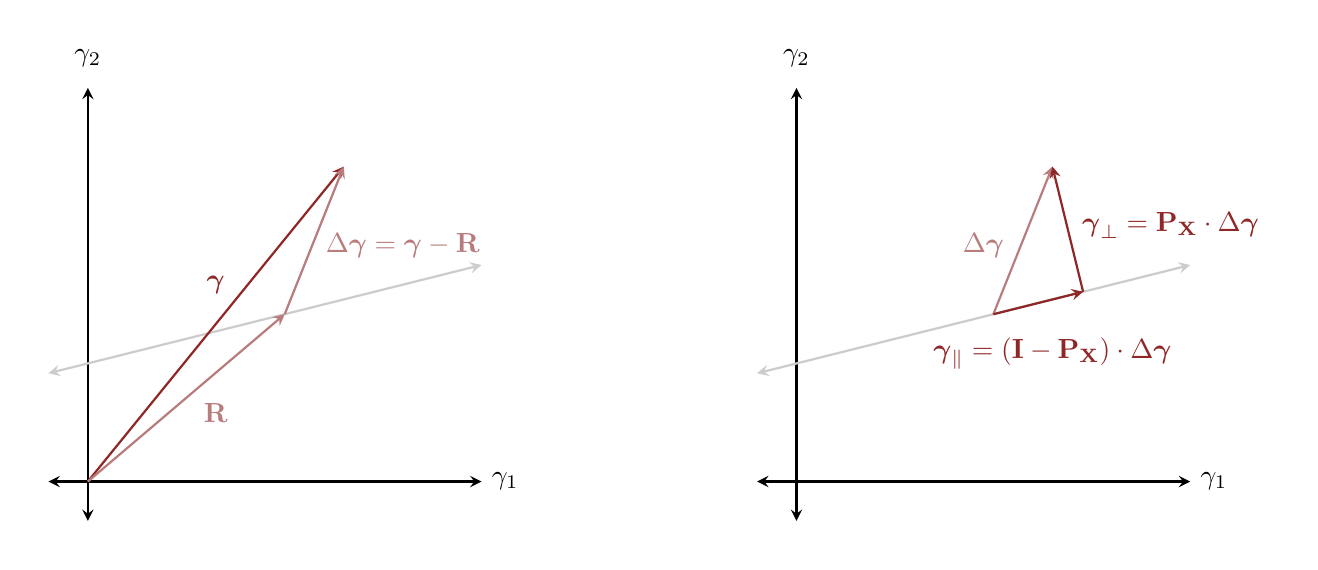
\begin{tikzpicture}[scale=0.5, thick]
  \draw[color=white] (-1.5, -1.5) rectangle +(14, 13);
  
  \draw[<->, >=stealth] (-1, 0) -- +(11, 0)
  node[right] { $\gamma_{1}$ };
  
  \draw[<->, >=stealth] (0, -1) -- +(0, 11);
  \node[] at (0, 10.75) { $\gamma_{2}$ };
  
  % y = 0.25 * x + 3
  \draw[<->, >=stealth, color=gray80] (-1, 2.75) -- (10, 5.5);
  
  \draw[color=dark,->, >=stealth] (0, 0) -- (6.5, 8);
  \node[color=dark] at (3.25, 5) { $\boldsymbol{\gamma}$ };
  
  \draw[color=mid,->, >=stealth] (0, 0) -- (5, 4.25);
  \node[color=mid] at (3.25, 1.75) { $\mathbf{R}$ };

  \draw[color=mid,->, >=stealth] (5, 4.25) -- (6.5, 8);
  \node[color=mid] at (8, 6) { $\Delta \boldsymbol{\gamma} = 
                                  \boldsymbol{\gamma} - \mathbf{R}$ };

  \pgfmathsetmacro{\dx}{18}

  \draw[color=white] (-1.5 + \dx, -1.5) rectangle +(14, 13);
  
  \draw[<->, >=stealth] (-1 + \dx, 0) -- +(11, 0)
  node[right] { $\gamma_{1}$ };
  
  \draw[<->, >=stealth] (0 + \dx, -1) -- +(0, 11);
  \node[] at (0 + \dx, 10.75) { $\gamma_{2}$ };
  
  % y = 0.25 * x + 3
  \draw[<->, >=stealth, color=gray80] (-1 + \dx, 2.75) -- (10 + \dx, 5.5);

  \draw[color=mid,->, >=stealth] (5 + \dx, 4.25) -- (6.5 + \dx, 8);
  \node[color=mid] at (4.75 + \dx, 6) { $\Delta \boldsymbol{\gamma}$ }; 

  \draw[color=dark,->, >=stealth] (5 + \dx, 4.25) -- (7.28 + \dx, 7.28 * 0.25 + 3);
  \node[color=dark] at (6.5 + \dx, 3.25) { $\boldsymbol{\gamma}_{\parallel} = 
    (\mathbf{I} - \mathbf{P}_{\mathbf{X}} ) \cdot \Delta \boldsymbol{\gamma}$ }; 

  \draw[color=dark,->, >=stealth] (7.28 + \dx, 7.28 * 0.25 + 3) -- (6.5 + \dx, 8);
  \node[color=dark] at (9.5 + \dx, 6.5) { $\boldsymbol{\gamma}_{\perp} = 
    \mathbf{P}_{\mathbf{X}} \cdot \Delta \boldsymbol{\gamma}$ }; 
    
\end{tikzpicture}

\end{document}  